\documentclass{if-beamer}
\usepackage{xcolor}
\setbeamertemplate{footline}[frame number]

%
% Choose how your presentation looks.
%
% For more themes, color themes and font themes, see:
% http://deic.uab.es/~iblanes/beamer_gallery/index_by_theme.html
%
\mode<presentation>
{
  \usetheme{default}      % or try Darmstadt, Madrid, Warsaw, ...
  \usecolortheme{default} % or try albatross, beaver, crane, ...
  \usefonttheme{default}  % or try serif, structurebold, ...
  \setbeamertemplate{navigation symbols}{}
  \setbeamertemplate{caption}[numbered]
} 
\usepackage{tikz}
\usetikzlibrary{shapes}
\usepackage{tcolorbox}
\usepackage[english]{babel}
\usepackage[utf8]{inputenc}
\usepackage[T1]{fontenc}
\usepackage{mathtools}
\newcommand{\defeq}{\vcentcolon=}
\newcommand{\eqdef}{=\vcentcolon}
\newcommand{\norm}[2]{\left\lVert#1\right\rVert_{#2}}
\DeclarePairedDelimiter{\ceil}{\lceil}{\rceil}
\newcommand*\circled[1]{\tikz[baseline=(char.base)]{
            \node[shape=circle,draw,inner sep=0.2pt] (char) {#1};}}
\newcommand\STAR{\raisebox{-.7em}{\tikz{\node[draw,star,star point height=.7em,minimum size=1em]{};} }}


\title[Neural Networks in Approximation]{Mathematical Techniques in the Approximation Theory that are Rooted in Neural Networks - Petersen}
\author{Ko, Suh, Huo}
\institute{Georgia Tech}
\date{Summer of 2020}
\graphicspath{{figures/}}

\begin{document}

\begin{frame}
  \titlepage
\end{frame}

% Uncomment these lines for an automatically generated outline.
%\begin{frame}{Outline}
%  \tableofcontents
%\end{frame}

\begin{frame}{Table of Contents}
\tableofcontents
    
\end{frame}

\section{Basics of Neural Networks}

\subsection{Definition}
\begin{frame}{Definition of Neural Network}

\vskip 0.5cm
We define neural network as a sequence of matrix-vector tuples:
\begin{itemize}
  \item $d, L \in \mathbb{N}$
  \item $N_0 = d, N_1, \dots, N_L \in \mathbb{N}, l \in \{1,\dots,L\}$
  \item $A_1, A_2, \dots, A_L \text{ such that } A_l \in \mathbb{R}^{N_l \times N_{l+1}}$
  \item $b_1, b_2, \dots, b_L \text{ such that } b_l \in \mathbb{R}^{N_l}$
  \item $\varrho: \mathbb{R} \to \mathbb{R}$
\end{itemize}
Then, a neural network is 
\begin{align*}
    \Phi = \big((A_1,b_1),(A_2, b_2),\dots,(A_L, b_L) \big)
\end{align*}
such that its realization $R(\Phi): \mathbb{R}^d \to \mathbb{R}^{N_L}$ is a function such that $R(\Phi)(x) = x_L$ where
\begin{align*}
    x_0 &\defeq x\\
    x_l &= \varrho(A_l x_{l-1} + b_l) \text{ for } l=1,\dots,L-1\\
    x_L &= A_{L} x_{l-1} + b_L
\end{align*}

\end{frame}

\subsection{Complexity of Neural Network}

\begin{frame}{Complexity of Neural Network}

\vskip 0.5cm
There are generally two ways of describing complexity of a neural network. Given the neural network $\Phi$ as above,
\begin{block}{Number of nonzero weights, layers, and neurons}
\begin{itemize}
    \item $M(\Phi) \defeq \sum_{j=1}^L (\norm{A_l}{0} + \norm{b_l}{0})$ (Number of nonzero weights)
    \item $L(\Phi) \defeq L$ (Number of layers)
    \item $N(\Phi) \defeq \sum_{k=0}^L N_k$ (Number of neurons)
\end{itemize}

\end{block}

\begin{block}{Quantization}
A neural network $\Phi$ is $(s,\varepsilon)$-quantized if all weights (elements of $A_i, b_i$ for $i\in\{1,\dots,L\}$) are elements of $$[-\epsilon^{-s}, \epsilon^{-s}] \cap 2^{-s\left\lceil\log _{2}(1 / \varepsilon)\right\rceil} \mathbb{Z}$$.
\end{block}
\end{frame}

\subsection{Operations of Neural Network}
\begin{frame}{Operations of Neural Network}
    \begin{block}{Realization of Identity}
        Let $\varrho$ be ReLU, let $d \in \mathbb{N}$ and define $$\Phi_d^{Id} \defeq \left((A_1,b_1),(A_2,b_2) \right) $$
        where 
        $$A_{1}:=\left(
        \begin{array}{c}
            \operatorname{Id}_{\mathbb{R}^{d}} \\
            -\operatorname{Id}_{\mathbb{R}^{d}}
        \end{array}
        \right) \quad b_{1}:=0, 
        \quad A_{2}:=\left(\operatorname{Id}_{\mathbb{R}^{d}} \quad-\operatorname{Id}_{\mathbb{R}^{d}}\right) \quad b_{2}:=0
        $$
    \end{block}
    Then, $\mathrm{R}_{\varrho}(\Phi_{d}^{\operatorname{Id}}) = \operatorname{Id}_{\mathbb{R}^d}$\\
    \medskip
    As a generalization, one can arbitrarily adjust the number of layers by adding arbitrary number of matrix-vector pairs $(\operatorname{Id}_{\mathbb{R}^{2d}}, 0)$ in between $(A_1,b_1)$ and $(A_2,b_2)$ above. This yields $\Phi_{d,L}^{\operatorname{Id}}$ with $L$ layers. Trivially, in case one wants $L=1$, $\Phi_{d,1}^{Id} \defeq \left((\operatorname{Id}_{\mathbb{R}^d}, 0) \right)$ suffices.
\end{frame}

\begin{frame}{Operations of Neural Networks}
    \begin{block}{Concatenation}
        {\small
        $\operatorname{Let} L_{1}, L_{2} \in \mathbb{N}$ and let $\Phi^{1}=\left(\left(A_{1}^{1}, b_{1}^{1}\right), \ldots,\left(A_{L_{1}}^{1}, b_{L_{1}}^{1}\right)\right)$ and $\Phi^{2}=\left(\left(A_{1}^{2}, b_{1}^{2}\right), \ldots,\left(A_{L_{2}}^{2}, b_{L_{2}}^{2}\right)\right)$
        be two neural networks such that the input layer of $\Phi^{1}$ has the same dimension as the output layer of
        $\Phi^{2} .$ Then, $\Phi^{1} \bullet \Phi^{2}$ denotes the following $L_{1}+L_{2}-1$ layer network:
        \begin{align*}
            \Phi^{1} \bullet \Phi^{2}:=\big(&\left(A_{1}^{2}, b_{1}^{2}\right), \ldots,\left(A_{L_{2}-1}^{2}, b_{L_{2}-1}^{2}\right),\left(A_{1}^{1} A_{L_{2}}^{2}, A_{1}^{1} b_{L_{2}}^{2}+b_{1}^{1}\right), \\
            &\left(A_{2}^{1}, b_{2}^{1}\right), \ldots,\left(A_{L_{1}}^{1}, b_{L_{1}}^{1}\right)\big)
        \end{align*}
        We call $\Phi^{1} \bullet \Phi^{2}$ the concatenation of $\Phi^{1}$ and $\Phi^{2}$
        }
    \end{block}
    \begin{block}{Sparse Concatenation}
        {\small
        Let $\varrho: \mathbb{R} \rightarrow \mathbb{R}$ be the ReLU, let $L_{1}, L_{2} \in \mathbb{N},$ and let $\Phi^{1}, \Phi^{2}$ be two neural networks as above. Let $\Phi_{d}^{\text {Id }}$ be as in the previous slide. Then, the sparse concatenation of
        $\Phi^{1}$ and $\Phi^{2}$ is defined as
        \[
        \Phi^{1} \odot \Phi^{2}:=\Phi^{1} \bullet \Phi_{d}^{\mathrm{id}} \bullet \Phi^{2}
        \]
        }
    \end{block}
\end{frame}

\begin{frame}{Operations of Neural Networks}
    \begin{block}{Properties of sparse concatenation}
        It follows immediately from above definitions that 
        {\small
        \begin{align*}
            \Phi^{1} \odot \Phi^{2}=\Big(&\left(A_{1}^{2}, b_{1}^{2}\right), \ldots,\left(A_{L_{2}-1}^{2}, b_{L_{2}-1}^{2}\right),\left(\left(\begin{array}{c}
            A_{L_{2}}^{2} \\
            -A_{L_{2}}^{2} \end{array}\right),\left(\begin{array}{c}
            b_{L_{2}}^{2} \\
            -b_{L_{2}}^{2}
            \end{array}\right)\right),\\
            &\left(\left[A_{1}^{1} \mid-A_{1}^{1}\right], b_{1}^{1}\right),\left(A_{2}^{1}, b_{2}^{1}\right), \ldots,\left(A_{L_{1}}^{1}, b_{L_{1}}^{1}\right)\Big)
        \end{align*}
        }
        Then, we can deduce the following properties:
        \begin{itemize}
            \item $L(\Phi^{1} \odot \Phi^{2}) = L_1 + L_2$
            \item $\mathrm{R}_{\varrho}\left(\Phi^{1} \odot \Phi^{2}\right)=\mathrm{R}_{\varrho}\left(\Phi^{1}\right) \circ \mathrm{R}_{\varrho}\left(\Phi^{2}\right)$
            \item $M\left(\Phi^{1} \odot \Phi^{2}\right) \leq 2 M\left(\Phi^{1}\right)+2 M\left(\Phi^{2}\right)$
        \end{itemize}
        Using the fact $ a+b \leq 2 \max \{a, b\}$ for $a, b \geq 0$, it follows inductively
        \[
        M\left(\Phi^{1} \odot \cdots \odot \Phi^{n}\right) \leq 4^{n-1} \cdot \max \left\{M\left(\Phi^{1}\right), \ldots, M\left(\Phi^{n}\right)\right\}
        \]
    \end{block}
\end{frame}

\begin{frame}{Operations of Neural Networks}
    
    \begin{block}{Parallelization}
        {\small
        Let $L \in \mathbb{N}$ and let $\Phi^{1}=\left(\left(A_{1}^{1}, b_{1}^{1}\right), \ldots,\left(A_{L}^{1}, b_{L}^{1}\right)\right)$ and $\Phi^{2}=\left(\left(A_{1}^{2}, b_{1}^{2}\right), \ldots,\left(A_{L}^{2}, b_{L}^{2}\right)\right)$ be
        two neural networks with L layers and with d-dimensional input. We define
        \[
        \mathrm{P}\left(\Phi^{1}, \Phi^{2}\right):=\left(\left(\widetilde{A}_{1}, \widetilde{b}_{1}\right), \ldots,\left(\widetilde{A}_{L}, \widetilde{b}_{L}\right)\right)
        \]
        where
        {\small
        \[
        \widetilde{A}_{1}:=\left(\begin{array}{c}
        A_{1}^{1} \\
        A_{1}^{2}
        \end{array}\right),\: \tilde{b}_{1}:=\left(\begin{array}{c}
        b_{1}^{1} \\
        b_{1}^{2}
        \end{array}\right) \quad \text { and } \quad \widetilde{A}_{\ell}:=\left(\begin{array}{cc}
        A_{\ell}^{1} & 0 \\
        0 & A_{\ell}^{2}
        \end{array}\right),\: \tilde{b}_{\ell}:=\left(\begin{array}{c}
        b_{\ell}^{1} \\
        b_{\ell}^{2}
        \end{array}\right)
        \]
        }
        for $ 1<\ell \leq L$. Then, $\mathrm{P}\left(\Phi^{1}, \Phi^{2}\right)$ is a neural network with d-dimensional input and $L$ layers, called the parallelization of
        $\Phi^{1}$ and $\Phi^{2}$.
        One can check $M\left(P\left(\Phi^{1}, \Phi^{2}\right)\right)=M\left(\Phi^{1}\right)+M\left(\Phi^{2}\right)$ and
        \[
        \mathrm{R}_{\varrho}\left(\mathrm{P}\left(\Phi^{1}, \Phi^{2}\right)\right)(x)=\left(\mathrm{R}_{\varrho}\left(\Phi^{1}\right)(x), \mathrm{R}_{\varrho}\left(\Phi^{2}\right)(x)\right) \quad \text { for all } x \in \mathbb{R}^{d}
        \]
    }
    \end{block}
    
    
\end{frame}

\begin{frame}{Parallelization}
    \begin{figure}[htbp]
        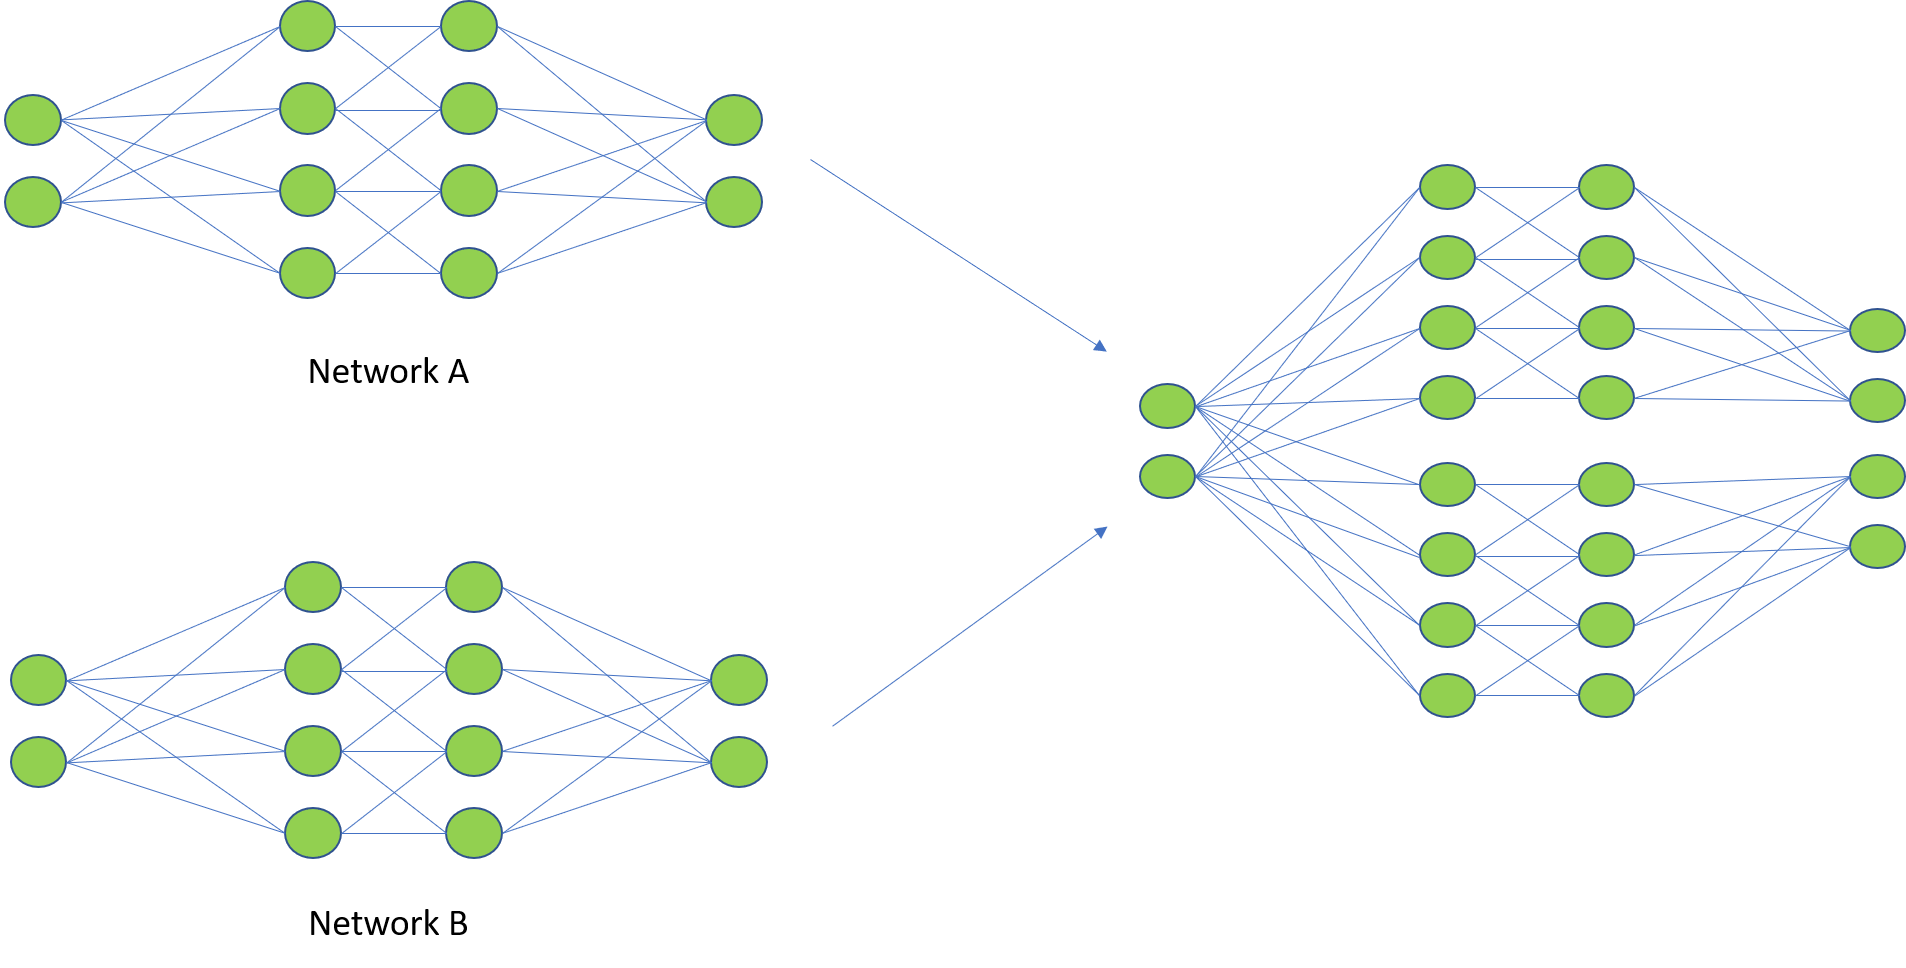
\includegraphics[width=1\textwidth]{parallelization.png}
        \caption{ Parallelization. }
        \label{fig:figure1}
    \end{figure}
\end{frame}

\section{Main}

\subsection{Mathematical Problem}
\begin{frame}{Mathematical Problem}
\begin{itemize}
    \item Given a function $f \in \mathcal{C}$ where $\mathcal{C}$ is some class of functions, how many weights, nodes, and layers does one need, and how much quantization do we require to approximate $f$ to $\varepsilon$ accuracy in some predefined metric?
\end{itemize}
\end{frame}

\subsection{Exemplary Results}
\begin{frame}{Exemplary Results}
    Suppose $f \in \mathcal{C} \subset L^{\infty}(\Omega)$.
    \begin{itemize}
        \item Barron; 1993: If $\mathcal{C}$ are bounded functions with one finite Fourier moment and $\varrho$ is sigmoidal, then there exist $\mathrm{NNs}\left(\Phi_{n}^{\rho}\right)_{n \in \mathbb{N}}$ such that $\left\|f-\Phi_{n}^{\varrho}\right\|_{L^{\infty}} \lesssim N\left(\Phi_{n}^{\varrho}\right)^{-1} \rightarrow 0$
        \item Mhaskar; 1993: For $\mathcal{C}=C^{s}\left([0,1]^{d}\right), \varrho$ a sigmoidal function of order $k \geq 2,$ and $L\left(\Phi_{n}^{\varrho}\right)=L(k, d, s),$ there exist $\mathrm{NNs}\left(\Phi_{n}^{\rho}\right)_{n \in \mathbb{N}}$ such that $\left\|f-\Phi_{n}^{\varrho}\right\|_{L^{\infty}} \lesssim N\left(\Phi_{n}^{\varrho}\right)^{-s / d} \rightarrow 0$
        \item Yarotsky; 2017: For $\mathcal{C}=C^{S}\left([0,1]^{d}\right)$ and $\varrho(x)=\max \{0, x\}$
        (called ReLU) and $L\left(\Phi_{n}^{\varrho}\right) \asymp \log (n)$ we have that there exist $\mathrm{NNs}$
        $\left(\Phi_{n}^{\varrho}\right)_{n \in \mathbb{N}}$ such that $\left\|f-\Phi_{n}^{\varrho}\right\|_{L^{\infty}} \lesssim W\left(\Phi_{n}^{\varrho}\right)^{-s / d} \rightarrow 0$
    \end{itemize}
\end{frame}

\section{Classifier Functions}
\subsection{Smooth Functions}
\begin{frame}{Smooth Functions}
    For a given $\beta \in (0,\infty)$ with $\beta = n + \sigma$ for $n \in \mathbb{N}_0, \sigma \in (0,1]$, let $f \in C^n([-\frac{1}{2}, \frac{1}{2}]^r)$. Define $$\|f\|_{C^{0, \beta}}:=\max \left\{\max _{|\alpha| \leq n}\left\|\partial^{\alpha} f\right\|_{\text {sup }}, \max _{|\alpha|=n} \operatorname{Lip}_{\sigma}(\partial f)\right\} \in[0, \infty] $$
    where \[
    \operatorname{Lip}_{\sigma}(g):=\sup _{x, y \in \Omega, x \neq y} \frac{|g(x)-g(y)|}{|x-y|^{\sigma}} \text { for } g: \Omega \subset \mathbb{R}^{d} \rightarrow \mathbb{R}
    \]
    Then, for $B>0,$ we define the following class of smooth functions:
    \[
    \mathcal{F}_{\beta, d, B}:=\left\{f \in C^{n}\left([-1 / 2,1 / 2]^{d}\right):\|f\|_{C^{0, \beta}} \leq B\right\}
    \]
\end{frame}

\subsection{Horizon Functions and Piecewise Constant Functions}
\begin{frame}{Horizon Functions and Piecewise Constant Functions}
    \begin{block}{Horizon functions}
        {\small
        We define the class of horizon functions as:
        \begin{align*}
            \mathcal{H F}_{\beta, d, B} := \{&f \circ T \in L^{\infty}\left([-1 / 2,1 / 2]^{d}\right): f(x)=H(x_{1}+\gamma\left(x_{2}, \ldots, x_{d}\right)\\ &,x_{2}, \ldots, x_{d}), \gamma \in \mathcal{F}_{\beta, d-1, B}, T \in \Pi(d, \mathbb{R})\}
        \end{align*}
        where $\Pi(d, \mathbb{R}) \subset G L(d, \mathbb{R})$ denotes the group of permutation matrices.
        }
    \end{block}
    \begin{block}{Piecewise constant functions}
        {\small
        Let $r \in \mathbb{N}$, $d \in \mathbb{N}_{\geq 2}$, and $\beta, B>0$. Define 
        \begin{align*}
            \mathcal{K}_{r, \beta, d, B}\defeq\{&K \subset[-1 / 2,1 / 2]^{d}: \forall x \in[-1 / 2,1 / 2]^{d}, \exists f_{x} \in \mathcal{H} \mathcal{F}_{\beta, d, B}:\\ &\chi_{K}=f_{x} \text { on }[-1 / 2,1 / 2]^{d} \cap \overline{B_{2^{-r}}}^{\|\cdot\|_{\ell^{\infty}}}(x)\}
        \end{align*}
        Then, the class of functions $\{\sum_{i \leq N}\chi_{K_i} : K_i \in \mathcal{K}_{r, \beta, d, B}, N \in \mathbb{N}\}$ characterizes piecewise constant functions.
        }
    \end{block}
\end{frame}

\subsection{Piecewise Smooth Functions}
\begin{frame}{Piecewise Smooth Functions}
    \begin{block}{Piecewise smooth functions}
        Finally, we consider the following class of piecewise smooth functions:
        $$
        \mathcal{E}_{r, \beta, d, B}^{p}:=\left\{f=\chi_{K} \cdot g: g \in \mathcal{F}_{\beta^{\prime}, d, B} \text { and } K \in \mathcal{K}_{r, \beta, d, B}\right\}
        $$
        Note that unlike in the case of piecewise constant functions, the smoothness of the boundary surface, $\beta$, is allowed to differ from the smoothness of smooth regions, $\beta'$.
    \end{block}
    \begin{block}{Approximation results}
        In the next set of slides, we study approximation capabilities of neural networks for the 4 classes of functions introduced above in the usual metric defined by $L^p$-norm in the domain $\left[-\frac{1}{2}, \frac{1}{2}\right]^d$.
    \end{block}
\end{frame}

\section{Approximation of Smooth Functions}
\subsection{Main Result}
\begin{frame}{Approximation of Smooth Functions \\(Theorem 3.1, P., Voigtlaender 2018)}
    \begin{tcolorbox}
        For any $d \in \mathbb{N},$ and $\beta, B, p>0,$ there exist constants $s=s(d, \beta, B, p) \in \mathbb{N}$ and $c=c(d, \beta, B)>0$ such that for any function $f \in \mathcal{F}_{\beta, d, B}$ and any $\varepsilon \in(0,1 / 2),$ there is a neural network $\Phi_{\varepsilon}^{f}$ with at most $\left(2+\left\lceil\log _{2} \beta\right\rceil\right) \cdot(11+\beta / d)$ layers, and at most $c \cdot \varepsilon^{-d / \beta}$ nonzero, $(s, \varepsilon)$ -quantized weights such that {\small
        \[
        \left\|\mathrm{R}_{\varrho}\left(\Phi_{\varepsilon}^{f}\right)-f\right\|_{L^{p}\left([-1 / 2,1 / 2]^{d}\right)}<\varepsilon \quad \text { and } \quad\left\|\mathrm{R}_{\varrho}\left(\Phi_{\varepsilon}^{f}\right)\right\|_{\mathrm{sup}} \leq\lceil B\rceil
        \]
        }
    \end{tcolorbox}
\end{frame}

\begin{frame}{Key Proof Ideas}
    \begin{itemize}
        \item Construct neural networks that can approximate multiplication, monomials, and polynomials up to arbitrary accuracy at the cost of some level of network complexity. (Lemma A.3, A.4, A.5)
        \item Construct an equally spaced $n$-dimensional grid on the domain of $f$, $[-\frac{1}{2}, \frac{1}{2}]^d$.
        \item Consider Taylor approximation of $f$ by $p_{i,\alpha}$ where $p_{i,\alpha}$ has $x_i$ in one of the grid cubes as its base point. (Lemma A.8)
        \item Construct a neural network whose number of outputs equals the number of grid cubes that can approximate any of $p_{i,\alpha}$ with one of its outputs. (Lemma A.5)
        \item Construct a neural network with 1-dimensional output that approximates each output of the network from previous step restricted to the corresponding grid cubes. (Lemma A.6, A.7)
        \item Modify the network from last step to ensure it has bounded outputs and make sure it satisfies all the stated properties regarding approximation accuracy, complexity, and number of layers. (Lemma A.1)
    \end{itemize}
\end{frame}

\begin{frame}{Bounding the Outputs of Neural Networks (Lemma A.1)}
    \begin{tcolorbox}
        There is a universal constant $c>0$ such that the following holds:\\
        For arbitrary $d, s, k \in \mathbb{N}, B>0, \varepsilon \in(0,1 / 2),$ and any neural network $\Psi$ with d-dimensional input and
        $k$ -dimensional output and with $(s, \varepsilon)$ -quantized weights, there exists a neural network $\Phi$ with the same input/output dimensions as $\Psi$ and with the following properties:\\
        {\small
        $\bullet$ \, $M(\Phi) \leq 2 M(\Psi)+c k,$ and $L(\Phi) \leq L(\Psi)+2$\\
        $\bullet$ All weights of $\Phi$ are $\left(s_{0}, \varepsilon\right)$ -quantized, where
        $$s_{0}:=\max \left\{\left\lceil\log _{2}(\lceil B\rceil)\right\rceil, s\right\}$$
        $\bullet$ \, $\mathrm{R}_{\varrho}(\Phi)=\left(\tau_{B} \times \cdots \times \tau_{B}\right) \circ \mathrm{R}_{\varrho}(\Psi),$ where the function
        \[
        \tau_{B}: \mathbb{R} \rightarrow[-\lceil B\rceil,\lceil B\rceil], y \mapsto \operatorname{sign}(y) \cdot \min \{|y|,\lceil B\rceil\}
        \]
        is $1$-Lipschitz and satisfies $\tau_{B}(y)=y$ for all $y \in \mathbb{R}$ with $|y| \leq\lceil B\rceil$
        }%
    \end{tcolorbox}
\end{frame}

\begin{frame}{Approximation of Multiplication (Lemma A.3)}
    \begin{tcolorbox}
        Let $\theta>0$ be arbitrary. Then, for every $L \in \mathbb{N}$ with $L>(2 \theta)^{-1}$ and each $M \geq 1$, there are constants $c=c(L, M, \theta) \in \mathbb{N}$ and $s=s(M) \in \mathbb{N}$ with the following property: For each $\varepsilon \in(0,1 / 2),$ there is a neural network $\widetilde{\times}$ with the following properties:\\
        $\bullet$ $\widetilde{\times}$ has at most $c \cdot \varepsilon^{-\theta}$ nonzero, $(s, \varepsilon)$-quantized weights;\\
        $\bullet$ $\widetilde{\times}$ has $2L+8$ layers;\\
        $\bullet$ $\forall x, y \in[-M, M],$ we have $\left|xy-\mathrm{R}_{\varrho}(\widetilde{x})(x, y)\right| \leq \varepsilon$\\
        $\bullet$  $\forall x, y \in[-M, M]$ with $x \cdot y=0,$ we have $\mathrm{R}_{\varrho}(\widetilde{x})(x, y)=0$
    \end{tcolorbox}
\end{frame}

\begin{frame}{Approximation of Monomials (Lemma A.4)}
    \begin{tcolorbox}
        Let $n, d, \ell \in \mathbb{N}$ be arbitrary. Then, there are constants $s=s(n) \in \mathbb{N}, c=c(d, n, \ell) \in \mathbb{N}$ and $L=L(d, n, \ell) \in \mathbb{N}$ such that $L \leq\left(1+\left\lceil\log _{2} n\right\rceil\right) \cdot(10+\ell / d)$ with the following property:\\
        For each $\varepsilon \in(0,1 / 2)$ and $\alpha \in \mathbb{N}_{0}^{d}$ with $|\alpha| \leq n,$ there is a neural network $\Phi_{\varepsilon}^{\alpha}$ with d-dimensional input
        and one-dimensional output, with at most $L$ layers, and with at most $c \cdot \varepsilon^{-d / \ell}$ nonzero, $(s, \varepsilon)$-quantized weights, and such that $\Phi_{\varepsilon}^{\alpha}$ satisfies
        \[
        \left|\mathrm{R}_{\varrho}\left(\Phi_{\varepsilon}^{\alpha}\right)(x)-x^{\alpha}\right| \leq \varepsilon
        \]
        for all $x \in\left[-\frac{1}{2}, \frac{1}{2}\right]^{d}$
    \end{tcolorbox}
\end{frame}

\begin{frame}{Approximation of Polynomials (Lemma A.5)}
    \begin{tcolorbox}
        Let $d, m \in \mathbb{N}$, let $B, \beta>0$,\\ 
        let $\left\{c_{\ell, \alpha}: \ell \in\{1, \ldots, m\}, \alpha \in \mathbb{N}_{0}^{d},|\alpha|<\beta\right\} \subset[-B, B]$ be a
        sequence of coefficients, and let $\left(x_{\ell}\right)_{\ell=1}^{m} \subset[-1 / 2,1 / 2]^{d}$ be a sequence of base points.\\
        Then, there exist constants $c=c(d, \beta, B)>0, s=s(d, \beta, B) \in \mathbb{N},$ and $L=L(d, \beta) \in \mathbb{N}$ with $L \leq 1+\left(1+\left\lceil\log _{2} \beta\right\rceil\right) \cdot(11+\beta / d)$ such that $\forall \varepsilon \in(0,1 / 2)$ there is a neural network $\Phi_{\varepsilon}^{\mathrm{p}}$ with at most $c \cdot\left(\varepsilon^{-d / \beta}+m\right)$ many nonzero, $(s, \varepsilon)$ -quantized weights, at most $L$ layers, and with an $m$ -dimensional output such that
        $\left|\left[\mathrm{R}_{\varrho}\left(\Phi_{\varepsilon}^{\mathrm{p}}\right)\right]_{\ell}(x)-\sum_{|\alpha|<\beta} c_{\ell, \alpha} \cdot\left(x-x_{\ell}\right)^{\alpha}\right|<\varepsilon \quad$ for all $\quad \ell \in\{1, \ldots, m\}$ and $x \in[-1 / 2,1 / 2]^{d}$
    \end{tcolorbox}
\end{frame}

\begin{frame}{Approximation of "cutoff" of a Network (Lemma A.6)}
    \begin{tcolorbox}
        Let$d \in \mathbb{N}, p \in(0, \infty),$ and $B \geq 1 .$ Let $-1 / 2 \leq a_{i} \leq b_{i} \leq 1 / 2$ for $i=1, \ldots, d,$ and let $\varepsilon \in(0,1 / 2)$ be arbitrary. Then there exist constants $c=c(d) \in \mathbb{N}, s=s(d, B, p) \in \mathbb{N},$ and a neural network $\Lambda_{\varepsilon}$ with a $d+1$ -dimensional input, at most four layers, and at most c nonzero, $(s, \varepsilon)$ -quantized weights such that for each neural network $\Phi$ with one-dimensional output layer and d-dimensional input layer, and with $\left\|\mathrm{R}_{\varrho}(\Phi)\right\|_{L^{\infty}\left([-1 / 2,1 / 2]^{d}\right)} \leq B,$ we have
        \[
        \left\|\mathrm{R}_{\varrho}\left(\Lambda_{\varepsilon}\right)\left(\bullet, \mathrm{R}_{\varrho}(\Phi)(\bullet)\right)-\chi_{\prod_{i=1}^{d}\left[a_{i}, b_{i}\right]} \cdot \mathrm{R}_{\varrho}(\Phi)\right\|_{L^{p}\left([-1 / 2,1 / 2]^{d}\right)} \leq \varepsilon
        \]
    \end{tcolorbox}
\end{frame}

\begin{frame}{Approximation of "cutoff" of a Network (Lemma A.7)}
    \begin{tcolorbox}
        Let $d, m, s \in \mathbb{N}, p \in(0, \infty),$ and $\varepsilon \in(0,1 / 2),$ and let $\Phi$ be a neural network with $d$ dimensional input and $m$ -dimensional output, and with $(s, \varepsilon)$-quantized weights. Furthermore, let $B \geq 1$ with $\left\|\left[\mathrm{R}_{\underline{\varrho}}(\Phi)\right]_{\ell}\right\|_{L^{\infty}\left([-1 / 2,1 / 2]^{d}\right)} \leq B$ for all $\ell=1, \ldots, m .$ Finally, let $-1 / 2 \leq a_{i, \ell} \leq b_{i, \ell} \leq 1 / 2$ for $i=1, \ldots, d$ and  $\ell=1, \ldots, m$.
        Then, there exist constants $c=c(d)>0, s_{0}=s_{0}(d, B, p) \in \mathbb{N},$ and a neural network $\Psi_{\varepsilon}$ with d-dimensional input layer and 1 -dimensional output layer, with at most $6+L(\Phi)$ layers, and at most $c \cdot(m+L(\Phi)+M(\Phi))$ nonzero, $\left(\max \left\{s, s_{0}\right\}, \varepsilon / m\right)$ -quantized weights, such that
        \[
        \| \mathrm{R}_{\varrho}\left(\Psi_{\varepsilon}\right)-\sum_{\ell=1}^{m} \chi_{\prod_{i=1}^{d}\left[a_{i, \ell}, b_{i, \ell}\right]} \cdot\left[\mathrm{R}_{\varrho}(\Phi)\right]_{\ell}||_{L^{p}\left([-1 / 2,1 / 2]^{d}\right)} \leq \varepsilon
        \]
    \end{tcolorbox}
\end{frame}

\begin{frame}{Taylor Approximation of Smooth Functions (Lemma A.8)}
    \begin{tcolorbox}
        Let $\beta \in(0, \infty),$ and write $\beta=n+\sigma$ with $n \in \mathbb{N}_{0}$ and $\sigma \in(0,1],$ and let $d \in \mathbb{N} .$ Then there is a constant $C=C(\beta, d)>0$ with the following property:\\
        For each $f \in \mathcal{F}_{\beta, d, B}$ and arbitrary $x_{0} \in(-1 / 2,1 / 2)^{d},$ there is a polynomial $p(x)=\sum_{|\alpha| \leq n} c_{\alpha}\left(x-x_{0}\right)^{\alpha}$ with $c_{\alpha} \in[-C \cdot B, C \cdot B]$ for all $\alpha \in \mathbb{N}_{0}^{d}$ with $|\alpha| \leq n$ and such that
        \[
        |f(x)-p(x)| \leq C \cdot B \cdot\left|x-x_{0}\right|^{\beta} \quad \text { for all } x \in[-1 / 2,1 / 2]^{d}
        \]
        In fact, $p=p_{f, x_{0}}$ is the Taylor polynomial of $f$ of degree $n$
    \end{tcolorbox}
    
\end{frame}


\section{Proof of Theorem 3.1}

\begin{frame}{Proof of Theorem 3.1}
    Set $p_0 \defeq \left\lceil p \right\rceil \in \mathbb{N}$. It suffices to show the result for approximation in $L^{p_0}$-norm since $\norm{f}{L^p\left([-1/2, 1/2]^{d}\right)} \leq \norm{f}{L^q\left([-1/2, 1/2]^{d}\right)}$ for $0<p\leq q <\infty$.\\
    Also, let $C=C(d, \beta) > 0$ be the constant from Lemma A.8 and define $N \defeq \left\lceil (\frac{\varepsilon}{4CBd^{\beta}})^{-\frac{1}{\beta}} \right\rceil \in \mathbb{N}$.\\
    Finally, for $\lambda \in \{1,\dots,N\}^d$, set $$I_{\lambda} \defeq \prod_{i=1}^d \left[ \frac{\lambda_i - 1}{N} - \frac{1}{2}, \frac{\lambda_i}{N} - \frac{1}{2} \right] $$
    Then, we have $$\left[-\frac{1}{2}, \frac{1}{2} \right]^d = \bigcup_{\lambda \in \{1,\dots,N\}^d}I_{\lambda} \text{ and } I_{\lambda} \subset \bar{B}_{1 / N}^{\|\cdot\|_{\ell^{\infty}}}(x) \subset \bar{B}_{d / N}^{|\cdot|}(x) \ \forall x \in I_{\lambda}  $$
\end{frame}


\begin{frame}{Proof of Theorem 3.1 (Continued 1)}
    Also, write $\{1,\dots, N \}^d = \{\lambda_1,\dots,\lambda_{N^d} \}$, and for each $i \in \{1,\dots,N^d \}$, choose $x_i \in interior(I_{\lambda_i})$ and set $c_{i,\alpha} \defeq \partial^{\alpha}f(x_i)/\alpha!$ for $\alpha \in \mathbb{N}_0^d$ with $|\alpha| \leq n$. Since $f \in \mathcal{F}_{\beta, d, B}$, $|c_{i,\alpha}| \leq B$.\\
    By Lemma A.8, we have $$ \sup _{i \in\left\{1, \ldots, N^{d}\right\}}\left|f(x)-p_{i, \alpha}(x)\right| \leq C B\left(\frac{d}{N}\right)^{\beta}$$ where $p_{i, \alpha}(x):=\sum_{|\alpha| \leq n} \frac{\partial^{\alpha} f\left(x_{i}\right)}{\alpha !}\left(x-x_{i}\right)^{\alpha}$, Taylor polynomial of $f$ of degree $n$.\\
    In particular, $$ |p_{i, \alpha}(x)| \leq |f(x)| + Cd^{\beta}B \leq \left\lceil (1+Cd^{\beta})B\right\rceil \eqdef B_1 \quad \forall x \in I_{\lambda_i}$$
\end{frame}

\begin{frame}{Proof of Theorem 3.1 (Continued 2)}
    For the polynomial defined above for each base point $(x_i)_{i=1,\dots,N^d}$, we can take $\Phi^p_{\varepsilon/4}$ by applying Lemma A.5 with $\varepsilon/4$ instead of $epsilon$ and with $m=N^d$. This network has at most $L_1 = L_1(d, \beta) \leq 1+\left(1+\left\lceil\log _{2} \beta\right\rceil\right) \cdot(11+\beta / d)$ layers and at most $c_1 \left(\varepsilon^{-d / \beta}+N^d\right)$ nonzero $(s_1, \varepsilon)$-quantized weights for some $c_1=c_1(d,\beta,B)>0$ and $s_1=s_1(d,\beta,B)\in \mathbb{N}$.\\
    Now apply Lemma A.1 with $B_1$ instead of $B$ to obtain a network $\Psi^p_{\varepsilon/4}$ such that 
    $$\mathrm{R}_{\varrho}\left(\Psi_{\varepsilon / 4}^{p}\right)=\left(\tau_{B_{1}} \times \cdots \times \tau_{B_{1}}\right) \circ \mathrm{R}_{\varrho}\left(\Phi_{\varepsilon / 4}^{P}\right)$$
    where $\tau_{B_{1}}: \mathbb{R} \rightarrow\left[-B_{1}, B_{1}\right]$ is 1-Lipschitz and satisfies $\tau_{B_{1}}(x)=x$ for all $x \in\left[-B_{1}, B_{1}\right]$ and has at most $L_2 \defeq L(\Psi_{\varepsilon / 4}^{p}) \leq 2 + L_1 \leq 3+\left(1+\left\lceil\log _{2} \beta\right\rceil\right)\cdot(11+\beta / d)$ and at most $2 c_{1} \cdot\left(\varepsilon^{-d / \beta}+N^{d}\right)+c_{2} \cdot N^{d} \leq c_{3} \cdot\left(\varepsilon^{-d / \beta}+N^{d}\right)$ nonzero, $\left(s_{2}, \varepsilon\right)$-quantized weights for an absolute constant $c_{2}>0$ and suitable $s_{2}=s_{2}(d, \beta, B) \in \mathbb{N}$ and $c_{3}=c_{3}(d, \beta, B)>0$. 
\end{frame}


\begin{frame}{Proof of Theorem 3.1 (Continued 3)}
    With these preparations, we have 
    \begin{align*}
        \left|\left[\mathrm{R}_{\varrho}\left(\Psi_{\varepsilon / 4}^{\mathrm{p}}\right)(x)\right]_{i}-p_{i, \alpha}(x)\right| &= \left|\tau_{B_{1}}\left(\left[\mathrm{R}_{\varrho}\left(\Phi_{\varepsilon / 4}^{\mathrm{p}}\right)\right]_i(x)\right)-\tau_{B_{1}}\left(p_{i, \alpha}(x)\right)\right|\\
        &\leq\left|\left[\mathrm{R}_{\varrho}\left(\Phi_{\varepsilon / 4}^{\mathrm{p}}\right)\right]_i(x)-p_{i, \alpha}(x)\right| \leq \frac{\varepsilon}{4}
    \end{align*}
    for all $x \in I_{\lambda_{i}}$ and $i \in\left\{1, \ldots, N^{d}\right\}$. Hence, we can write
    {\small
    \begin{align*}
        \norm{f-\sum_{i \in\{1, \ldots, N^{d}\}} \chi_{I_{\lambda_{i}}}\left[\mathrm{R}_{\varrho}\left(\Psi_{\varepsilon / 4}^{\mathrm{p}}\right)\right]_{i}}{L^{\infty}} & \leq \sup _{i \in\left\{1, \ldots, N^{d}\right\}}\left|f(x)-\left[\mathrm{R}_{\varrho}\left(\Psi_{\varepsilon / 4}^{\mathrm{p}}\right)\right]_{i}(x)\right| \\
        & \leq \frac{\varepsilon}{4}+\sup _{x \in I_{\lambda_{i}}}\left|f(x)-p_{i, \alpha}(x)\right|\\ 
        &\leq \frac{\varepsilon}{4}+C B\left(\frac{d}{N}\right)^{\beta} \\
        &\leq \frac{\varepsilon}{2}
    \end{align*}
    }%
\end{frame}

\begin{frame}{Proof of Theorem 3.1 (Continued 4)}
    Now, apply Lemma A.7 with $\varepsilon/2$ instead of $\varepsilon$, $p_0$ instead of $p$, $\Phi = \Psi^p_{\varepsilon/4}$, $m=N^d$, and $\prod_{i=1}^{d}\left[a_{i, \ell}, b_{i, \ell}\right] = I_{\lambda_{\ell}}$ to obtain a network $\Psi_{\varepsilon}$ such that $\left\|\mathrm{R}_{\varrho}\left(\Psi_{\varepsilon}\right)-\sum_{i \in\left\{1, \ldots, N^{d}\right\}} \chi_{I_{\lambda_{i}}}\left[\mathrm{R}_{\varrho}\left(\Psi_{\varepsilon / 4}^{\mathrm{p}}\right)\right]_{i}\right\|_{L^{p_{0}}} \leq \frac{\varepsilon}{2}$\\
    Then $\Psi_{\varepsilon}$ has at most $3 + L_2 \leq 9 + \left(1+\left\lceil\log _{2} \beta\right\rceil\right)\cdot(11+\beta / d)$ layers and at most 
    \begin{align*}
        c_{4} \cdot\left(N^{d}+L\left(\Psi_{\varepsilon / 4}^{\mathrm{p}}\right)+M\left(\Psi_{\varepsilon / 4}^{\mathrm{p}}\right)\right) &\leq c_{4} \cdot\left(N^{d}+L_{2}+M\left(\Psi_{\varepsilon / 4}^{\mathrm{p}}\right)\right)\\ &\leq c_{5} \cdot\left(N^{d}+c_{3}\left(\varepsilon^{-d / \beta}+N^{d}\right)\right)
    \end{align*}
    nonzero, $\left(\max \left\{s_{2}, s_{0}\right\}, \varepsilon /\left(2 N^{d}\right)\right)$-quantized weights, with constants $c_{4}=c_{4}(d)>0, c_{5}=c_{5}(d, \beta)>0$ and $s_0=s_0(d,B,p)$.\\
    By using the inequality $\varepsilon/(2N^d) \geq c_7\cdot \varepsilon^{1+d/\beta}$ for some $c_7 = c_7(d,\beta,B)$, we can conclude that the weights of $\Psi_{\varepsilon}$ is $(s,\varepsilon)$-quantized for $s=s(d,\beta,p,B)$
\end{frame}

\begin{frame}{Proof of Theorem 3.1 (Continued 5)}
    Note that $\Psi_{\varepsilon}$ now satisfies 
    {\small
    \begin{align*}
        \left\|f - \mathrm{R}_{\varrho}\left(\Psi_{\varepsilon}\right)\right\|_{L^{p_{0}}([-\frac{1}{2}, \frac{1}{2}]^d)} &\leq
         \norm{f-\sum_{i \in\{1, \ldots, N^{d}\}} \chi_{I_{\lambda_{i}}}\left[\mathrm{R}_{\varrho}\left(\Psi_{\varepsilon / 4}^{\mathrm{p}}\right)\right]_{i}}{L^{\infty}}\\
         &+ \left\|\mathrm{R}_{\varrho}\left(\Psi_{\varepsilon}\right)-\sum_{i \in\left\{1, \ldots, N^{d}\right\}} \chi_{I_{\lambda_{i}}}\left[\mathrm{R}_{\varrho}\left(\Psi_{\varepsilon / 4}^{\mathrm{p}}\right)\right]_{i}\right\|_{L^{p_{0}}([-\frac{1}{2}, \frac{1}{2}]^d)} \\
         &\leq \frac{\varepsilon}{2} + \frac{\varepsilon}{2} = \varepsilon
    \end{align*}
    }%
    Lastly, we apply Lemma A.1 to $\Psi_{\varepsilon}$ to obtain $\Phi_{\varepsilon}^f$ so that $$\mathrm{R}_{\varrho}(\Phi_{\varepsilon}^f) = \tau_B \circ \mathrm{R}_{\varrho}(\Psi_{\varepsilon}) $$
    Since, $\norm{f}{\sup} \leq B$, we have $f = \tau_B \circ f$ so that $$\norm{\mathrm{R}_{\varrho}(\Phi_{\varepsilon}^f) - f}{L^{p_0}([-\frac{1}{2}, \frac{1}{2}]^d)} \leq  \norm{\mathrm{R}_{\varrho}(\Psi_{\varepsilon}) - f}{L^{p_0}([-\frac{1}{2}, \frac{1}{2}]^d)} \leq \varepsilon$$
    It is easy to see that $\Phi_{\varepsilon}^f$ satisfies all the properties stated in the theorem. \qed
\end{frame}

\subsection{Approximation of Horizon Functions}
\begin{frame}{Approximation of Horizon Functions \\ (Lemma 3.4, P., Voigtlaender 2018)}
    \begin{tcolorbox}
        For any $p, \beta, B>0$ and $d \in \mathbb{N}_{\geq 2}$ there exist constants $c=c(d, \beta, B, p)>0,$ and $s=s(d, \beta, B, p) \in \mathbb{N},$ such that for every function $f \in \mathcal{H} \mathcal{F}_{\beta, d, B}$ and every $\varepsilon \in(0,1 / 2)$ there is $a$ neural network $\Phi_{\varepsilon}^{f}$ with at most $\left(2+\left\lceil\log _{2} \beta\right\rceil\right) \cdot(14+2 \beta / d)$ layers, and at most $c \cdot \varepsilon^{-p(d-1) / \beta}$ nonzero,
        $(s, \varepsilon)$-quantized weights, such that $\left\|\mathrm{R}_{\varrho}\left(\Phi_{\varepsilon}^{f}\right)-f\right\|_{L^{p}\left([-1 / 2,1 / 2]^{d}\right)}<\varepsilon .$ Moreover, $0 \leq \mathrm{R}_{\varrho}\left(\Phi_{\varepsilon}^{f}\right)(x) \leq 1$ for all
        $x \in \mathbb{R}^{d}$    
    \end{tcolorbox}
\end{frame}

\begin{frame}{Approximation of Heaviside function (Lemma A.2)}
    \begin{tcolorbox}
        Let $d \in \mathbb{N}_{\geq 2}$ and $H:=\chi_{[0, \infty) \times \mathbb{R}^{d-1}}$. For every $\varepsilon>0$ there exists a neural network $\Phi_{\varepsilon}^{H}$ with two layers and five (nonzero) weights which only take values in $\left\{\varepsilon^{-1}, 1,-1\right\},$ such that $0 \leq \mathrm{R}_{\varrho}\left(\Phi_{\varepsilon}^{H}\right) \leq 1 \quad$ and $\quad\left|H(x)-\mathrm{R}_{\varrho}\left(\Phi_{\varepsilon}^{H}\right)(x)\right| \leq \chi_{[0, \varepsilon] \times \mathbb{R}^{d-1}}(x) \quad$ for all $\quad x \in \mathbb{R}^{d}$ Moreover, $\left\|H-\mathrm{R}_{\varrho}\left(\Phi_{\varepsilon}^{H}\right)\right\|_{L^{p}\left([-1 / 2,1 / 2]^{d}\right)} \leq \varepsilon^{1 / p}$ for all $p \in(0, \infty)$
    \end{tcolorbox}
\end{frame}

\begin{frame}{Proof of Lemma 3.4}
    Write $f=H \circ \Tilde{\gamma}$ where 
    {\small
    $$\widetilde{\gamma}(x)=\left(x_{1}+\gamma\left(x_{2}, \ldots, x_{d}\right), x_{2}, \ldots, x_{d}\right) \text { for } x=\left(x_{1}, \ldots, x_{d}\right) \in\left[-\frac{1}{2},\frac{1}{2}\right]^{d} $$
    }%
    where $\gamma \in \mathcal{F}_{\beta, d-1,   B}$.  \\
    Apply Theorem 3.1 to approximate $\gamma$ with $p=1$, $d-1$ instead of $d$, and $\frac{1}{2}\cdot \left(\frac{\varepsilon}{4}\right)^p$ instead of $\varepsilon$. This yields a network $\Phi_{\varepsilon}^{\gamma}$ with at most 
    {\small $$L=L(d,\beta) \leq 11+ \left(1+\left\lceil\log _{2} \beta\right\rceil\right) \cdot(11+\frac{\beta}{d-1}) \leq 11+\left(1+\left\lceil\log _{2} \beta\right\rceil\right) \cdot(11+\frac{2\beta}{d})$$ }
    layers and at most $c \cdot \varepsilon^{-p(d-1)/\beta}$ nonzero, $(s, \varepsilon)$-quantized weights for $c = c(d,\beta,B,p) >0$ and $s=s(d, \beta, B, p)$ such that
    $$ \norm{\mathrm{R}_{\varrho}(\Phi_{\varepsilon}^{\gamma}) - \gamma}{L^1} \leq \frac{1}{2}\cdot \left(\frac{\varepsilon}{4} \right)^p
    $$
    Then, denote $\gamma_{\varepsilon} \defeq \mathrm{R}_{\varrho}(\Phi_{\varepsilon}^{\gamma})$
\end{frame}

\begin{frame}{Proof of Lemma 3.4 (Continued 1)}
    Clearly, one can construct $\Phi_{\varepsilon}^{\widetilde{\gamma}}$ with same number of nonzero weights and quantization (up to multiplicative constant dependent on $d, \beta$) and $L(\Phi_{\varepsilon}^{\widetilde{\gamma}}) \leq 1 + L(\Phi_{\varepsilon}^{\gamma})$ such that
    $$ \mathrm{R}_{\varrho}\left(\Phi_{\varepsilon}^{\widetilde{\gamma}} \right)(x) = \left(x_1 + \gamma_{\varepsilon}(x_2,\dots,x_d),x_2,\dots,x_d \right) \quad \forall x \in \mathbb{R}^d $$
    As a second step, apply Lemma A.2 with $\varepsilon' \in 2^{-\mathbb{N}}$ such that $\frac{1}{4}\cdot \left(\frac{\varepsilon}{4} \right)^p \leq \varepsilon' \leq \frac{1}{2}\cdot \left(\frac{\varepsilon}{4} \right)^p$ to obtain $\Phi_{\varepsilon'}^H$ with two layers and 5 nonzero weights such that $$\left|H(x) - \mathrm{R}_{\varrho}\left(\Phi_{\varepsilon'}^H \right)\right| \leq \chi_{[0, \varepsilon'] \times \mathbb{R}^{d-1}}(x) $$ 
    and $0 \leq\mathrm{R}_{\varrho}\left(\Phi_{\varepsilon'}^H \right) \leq 1$. We also have that all weights of $\Phi_{\varepsilon'}^H$ belong to $[-4(\varepsilon/4)^{-p}, 4(\varepsilon/4)^{-p}] \cap \mathbb{Z} \subset [-\varepsilon^{-s'}, \varepsilon^{-s'}] \cap \mathbb{Z}$ where $s' \defeq 2+3\lceil p \rceil$.
\end{frame}

\begin{frame}{Proof of Lemma 3.4 (Continued 2)}
    Now we concatenate two networks above to get $\Phi_{\varepsilon'}^H \odot \Phi_{\varepsilon}^{\widetilde{\gamma}}$ with at most $\widetilde{L} \leq 2 + L(\Phi_{\varepsilon}^{\widetilde{\gamma}}) \leq 14 + \left(1+\left\lceil\log _{2} \beta\right\rceil\right) \cdot(11+\frac{2\beta}{d})$ layers and no more than $\widetilde{c}\cdot \varepsilon^{-p(d-1)/\beta}$ nonzero $(s'',\varepsilon)$-quantized weights for suitable $s''=s''(d,\beta,B,p) \in \mathbb{N}$. Clearly, $0 \leq \mathrm{R}_{\varrho}(\Phi_{\varepsilon'}^H \odot \Phi_{\varepsilon}^{\widetilde{\gamma}}) \leq 1$.\\
    Now, we check that $\mathrm{R}_{\varrho}(\Phi_{\varepsilon'}^H \odot \Phi_{\varepsilon}^{\widetilde{\gamma}})$ approximates $f = H \circ \widetilde{\gamma}$ with $L^p$-error at most $\varepsilon$.\\
    Now, observe that for $q \defeq 1+\frac{1}{p} \geq max\{1, \frac{1}{p}\}$,
    {\small 
    \begin{align*}
        \norm{H \circ \widetilde{\gamma} - \mathrm{R}_{\varrho}(\Phi_{\varepsilon'}^H \odot \Phi_{\varepsilon}^{\widetilde{\gamma}})}{L^p} 
        = \norm{H \circ \widetilde{\gamma} - \mathrm{R}_{\varrho}(\Phi_{\varepsilon'}^H) \circ \mathrm{R}_{\varrho}(\Phi_{\varepsilon}^{\widetilde{\gamma}})}{L^p}\\
        \leq 2^q \cdot \max\left\{\norm{H \circ \widetilde{\gamma} - H \circ \mathrm{R}_{\varrho}(\Phi_{\varepsilon'}^H)}{L^p}, \norm{H \circ \mathrm{R}_{\varrho}(\Phi_{\varepsilon'}^H) -\mathrm{R}_{\varrho}(\Phi_{\varepsilon'}^H \odot \Phi_{\varepsilon}^{\widetilde{\gamma}}) }{L^p} \right\} \\
        \eqdef 2^q \cdot \max \{I,II \}
    \end{align*}}%
    From now, write $\chi_{\widetilde{\gamma}}$ to denote indicator function of the set $\{x \in [-1/2, 1/2]^d: \widetilde{\gamma}(x)>0 \}$, and we write $\mathrm{R}_{\varrho}(\Phi_{\varepsilon}^{\widetilde{\gamma}})_1$ to denote the first coordinate of the value $\mathrm{R}_{\varrho}(\Phi_{\varepsilon}^{\widetilde{\gamma}})$.
\end{frame}

\begin{frame}{Proof of Lemma 3.4 (Continued 3)}
    We first bound $I$ from above.\\
    {\small
    \begin{align*}
        &(2^q \cdot I)^p = 2^{1+p}\cdot \norm{H \circ \widetilde{\gamma} - H \circ \mathrm{R}_{\varrho}(\Phi_{\varepsilon'}^H) }{L^p}^p\\
        &= 2^{1+p} \int_{[-1/2,1/2]^d} \left|\chi_{\widetilde{\gamma}_1\geq 0}\left(x\right) - \chi_{\mathrm{R}_{\varrho}(\Phi_{\varepsilon'}^H)_1 \geq 0}\left(x\right)\right|^p dx\\
        &= 2^{1+p} \int_{[-\frac{1}{2},\frac{1}{2}]^{d-1}} \int_{-\frac{1}{2}}^{\frac{1}{2}} \chi_{\widetilde{\gamma}_1\geq 0, \mathrm{R}_{\varrho}(\Phi_{\varepsilon'}^H)_1 < 0}(x_1,\dots,x_d) \\
        & \qquad \qquad \qquad \qquad \qquad + \chi_{\widetilde{\gamma}_1< 0, \mathrm{R}_{\varrho}(\Phi_{\varepsilon'}^H)_1 \geq 0}(x_1,\dots,x_d)dx_1d(x_2,\dots,x_d)
    \end{align*}
    }%
    Then, since 
    {\small
    \begin{align*}
    \chi_{\widetilde{\gamma}_1 \geq 0, \mathrm{R}_{\varrho}(\Phi_{\varepsilon'}^H)_1 < 0} = 1
    &\iff x_1 + \gamma(x_2,\dots,x_d)\geq 0 \text{ and } x_1 + \gamma_{\varepsilon}(x_2,\dots,x_d)<0\\
    &\iff x_1 \in [-\gamma(x_2,\dots,x_d), -\gamma_{\varepsilon}(x_2,\dots,x_d)) 
    \end{align*}
    }%
    we have
    {\small
    $$\int_{-\frac{1}{2}}^{\frac{1}{2}} \chi_{\widetilde{\gamma}_1\geq 0, \mathrm{R}_{\varrho}(\Phi_{\varepsilon'}^H)_1 < 0}(x_1,\dots,x_d) dx_1 \leq \max \{0,\gamma(x_2,\dots,x_d)-\gamma_{\varepsilon}(x_2,\dots,x_d) \}$$
    }%
\end{frame}

\begin{frame}{Proof of Lemma 3.4 (Continued 4)}
    By similar reasoning, we also have
    {\small
    $$\int_{-\frac{1}{2}}^{\frac{1}{2}} \chi_{\widetilde{\gamma}_1< 0, \mathrm{R}_{\varrho}(\Phi_{\varepsilon'}^H)_1 \geq 0}(x_1,\dots,x_d) dx_1 \leq \max \{0,\gamma_{\varepsilon}(x_2,\dots,x_d) - \gamma(x_2,\dots,x_d)\}$$
    }%
    Hence,
    {\small
    \begin{align*}
    (2^q \cdot I)^p &\leq 2^{1+p}\int_{[-\frac{1}{2},\frac{1}{2}]^{d-1}}\max\{0, \gamma(y) - \gamma_{\varepsilon}(y)\} + \max\{0, \gamma_{\varepsilon} - \gamma(y)\}dy\\
    &= 2^{1+p}\norm{\gamma - \gamma_{\varepsilon}}{L^1([-\frac{1}{2}, \frac{1}{2}]^{d-1})}\\
    &\leq \left(\frac{\varepsilon}{2}\right)^p
    \end{align*}
    }%
    This shows $2^q \cdot I \leq \frac{\varepsilon}{2}$.\\
    Now we bound $II$. By construction of $\mathrm{R}_{\varrho}(\Phi_{\varepsilon'}^H)$, we have $|H(x) - \mathrm{R}_{\varrho}(\Phi_{\varepsilon'}^H)(x)| \leq \chi_{[0, \varepsilon'] \times \mathbb{R}^{d-1}}(x) \leq \chi_{[0, \frac{1}{2}(\frac{\varepsilon}{4})^p] \times \mathbb{R}^{d-1}}(x)$ $\forall x \in \mathbb{R}^d$.
\end{frame}

\begin{frame}{Proof of Lemma 3.4 (Continued 5)}
    Therefore, we can write
    {\small
    \begin{align*}
        (2^q \cdot II)^p &\leq 2^{1+p} \int_{[-\frac{1}{2},\frac{1}{2}]^{d}} \chi_{0\leq \mathrm{R}_{\varrho}(\Phi_{\varepsilon}^{\widetilde{\gamma}})_1 \leq \frac{1}{2}(\frac{\varepsilon}{4})^p] \times \mathbb{R}^{d-1}}(x)\\
        &= 2^{1+p} \int_{[-\frac{1}{2},\frac{1}{2}]^{d-1}} \int_{-\frac{1}{2}}^{\frac{1}{2}} \chi_{0\leq x_1+\gamma_{\varepsilon}(x_2,\dots,x_d)\leq \frac{1}{2}(\varepsilon/4)^p} dx_1 d(x_2,\dots,x_d)\\
        &\leq 2^p \int_{[-\frac{1}{2},\frac{1}{2}]^{d-1}}(\varepsilon/4)^p d(x_2,\dots,x_d) = (\varepsilon/2)^p
    \end{align*}
    }%
    from which we can conclude $2^q \cdot II \leq \varepsilon/2$.\\
    Hence,
    {\small
    $$ \norm{H \circ \widetilde{\gamma} - \mathrm{R}_{\varrho}(\Phi_{\varepsilon'}^H \odot \Phi_{\varepsilon}^{\widetilde{\gamma}})}{L^p} \leq 2^q \cdot \max\{I, II\} \leq \varepsilon/2 < \varepsilon$$
    }%
    Finally, noting that we can change coordinates by applying a permutation matrix to $A_1$ for any neural network $\Phi = ((A_1,b_1), \dots, (A_L,b_L)$ without changing number of layers, number of nonzero weights, and quantization, we see that we can assume $T$ in the definition of $\mathcal{HF}_{\beta,d,B}$ to be the identity matrix without loss of generality, so we're done. \qed 
\end{frame}

\subsection{Approximation of Piecewise Constant Functions}
\begin{frame}{Approximation of Piecewise Constant Functions \\ (Theorem 3.5 P., Voigtlaender 2018)}
    \begin{tcolorbox}
    For $r \in \mathbb{N}, d \in \mathbb{N}_{\geq 2},$ and $p, \beta, B>0,$ there are constants $c=c(d, r, p, \beta, B)>0$ and $s=s(d, r, p, \beta, B) \in \mathbb{N},$ such that for any $K \in \mathcal{K}_{r, \beta, d, B}$ and any $\varepsilon \in(0,1 / 2),$ there is a neural network $\Phi_{\varepsilon}^{K}$ with at most $\left(3+\left\lceil\log _{2} \beta\right\rceil\right) \cdot(11+2 \beta / d)$ layers, and at most $c \cdot \varepsilon^{-p(d-1) / \beta}$ nonzero, $(s, \varepsilon)$-quantized weights such that {\small
    \[
    \left\|\mathrm{R}_{\varrho}\left(\Phi_{\varepsilon}^{K}\right)-\chi_{K}\right\|_{L^{p}\left([-1 / 2,1 / 2]^{d}\right)}<\varepsilon \quad \text { and } \quad\left\|\mathrm{R}_{\varrho}\left(\Phi_{\varepsilon}^{K}\right)\right\|_{\text {sup }} \leq 1
    \]}
    \end{tcolorbox}
\end{frame}

\begin{frame}{Proof of Theorem 3.5}
    For $\lambda=\left(\lambda_{1}, \ldots, \lambda_{d}\right) \in\left\{1, \ldots, 2^{r}\right\}^{d},$ define
    \[
    I_{\lambda}:=\prod_{i=1}^{d}\left[\left(\lambda_{i}-1\right) \cdot 2^{-r}-\frac{1}{2}, \lambda_{i} \cdot 2^{-r}-\frac{1}{2}\right]
    \]
    We have by construction (with disjointness up to null sets) that
    $[-1 / 2,1 / 2]^{d}=\bigcup_{\lambda \in\left\{1, \ldots, 2^{r}\right\}^{d}} I_{\lambda}, \quad$ and $\quad I_{\lambda} \subset \bar{B}_{2^{-r}}^{\|\cdot\|_{e^{\infty}}}(x)$ for all $\quad x \in I_{\lambda}$.\\
    Then, by definition of $\mathcal{K}_{r,\beta,d,B}$, for each $\lambda \in \left\{1, \ldots, 2^{r}\right\}^{d}$, $\exists f_{\lambda} \in \mathcal{HF}_{\beta, d, B}$ such that $\chi_{I_{\lambda}} \chi_{K} = \chi_{I_{\lambda}}f_{\lambda}$\\
    Applying Lemma 3.4 to each $f_{\lambda}$, we get $\Phi_{\varepsilon}^{\lambda}$ such that
    {\small
    $$\left\|\mathrm{R}_{\varrho}\left(\Phi_{\varepsilon}^{\lambda}\right)-f_{\lambda}\right\|_{L^{p}} \leq \frac{\varepsilon}{2^{1+q+r d q}} \quad \text { and } \quad 0 \leq \mathrm{R}_{\varrho}\left(\Phi_{\varepsilon}^{\lambda}\right)(x) \leq 1 \quad \forall x \in \mathbb{R}^{d}
    $$
    }%
    and $\Phi_{\varepsilon}^{\lambda}$ has at most $L_1 \leq 14+\left(1+\left\lceil\log _{2} \beta\right\rceil\right) \cdot(11+\frac{2\beta}{d})$ layers and at most $c_1\cdot \varepsilon^{p(d-1)/\beta}$ nonzero, $(s_1, \varepsilon)$-quantized weights for $L_1 = L_1(d,\beta), c_1 = c_1(d,\beta, B, r, p)>0, s_1=s_1(d,\beta,B,r,p) \in \mathbb{N}$ 
\end{frame}

\begin{frame}{Proof of Theorem 3.5 (Continued 1)}
    There is no problem in assuming $\Phi_{\varepsilon}^{\lambda}$ has exactly $L_1$ layers by using sparse concatenation with identity network, and we'd still have same order of complexity and number of layers.\\
    Then, we can parallelize all of $\Phi_{\varepsilon}^{\lambda}$ to obtain 
    $$\Phi \defeq P(\Phi_{\varepsilon}^{\lambda_1}, P(\Phi_{\varepsilon}^{\lambda_2}, \dots, P(\Phi_{\varepsilon}^{\lambda_{2^{rd}-1}},\Phi_{\varepsilon}^{\lambda_{2^{rd}}})\dots))$$
    Apply Lemma A.7 with $m=2^{rd}, B=1$ with $\varepsilon/(2^{1+q})$ instead of $\varepsilon$ and with $I_{\lambda_l}$ for $l \in \{1,\dots,2^{rd}\}$ to obtain $\Psi$ that satisfies
    {\footnotesize
    \begin{align*}
        &\norm{\mathrm{R}_{\varrho}(\Psi) - \chi_{K}}{L^p} = \norm{\mathrm{R}_{\varrho}(\Psi) - \sum_{l \in \{1,\dots,2^{rd} \}}\chi_{I_{\lambda_l}} f_{\lambda_l}}{L^p}\\
        &\leq 2^q \norm{\mathrm{R}_{\varrho}(\Psi) - \sum_{l \in \{1,\dots,2^r \}}\chi_{I_{\lambda_l}} \left[\mathrm{R}_{\varrho}(\Phi)\right]_l}{L^p} + 2^q \norm{\sum_{l \in \{1,\dots,2^{rd} \}}\chi_{I_{\lambda_l}}\left( \left[\mathrm{R}_{\varrho}(\Phi)\right]_l - f_{\lambda_l} \right)}{L^p}\\
        &\leq \frac{\varepsilon}{2} + 2^{q+rdq}\cdot \max_{l\in\{1,\dots,2^{rd}\}}\left\{ \norm{\mathrm{R}_{\varrho}(\Phi_{\varepsilon}^{\lambda_l}) - f_{\lambda_l}}{L^p} \right\} \leq \varepsilon
    \end{align*}
    }%
\end{frame}

\begin{frame}{Proof of Theorem 3.5 (Continued 2)}
    By properties of parallelization, we observe $\Phi$ has $L_1$ layers and at most $2^{rd}\cdot c_1 \cdot \varepsilon^{p(d-1)/\beta}$ nonzero $(s_1,\varepsilon)$-quantized weights.\\
    By Lemma A.7, $\Psi$ has at most $6 + L(\Phi) = 6 + L_1$ layers and $(\max\{s_0, s_1\}, \varepsilon/(2^{1+q}))$-quantized weights so that we can say it is also $(s_2, \varepsilon)$-quantized for $s_2 = s_2(d,\beta,B,r,p)\in \mathbb{N}$. Finally, $M(\Psi) \leq c \cdot (2^{rd} + L_1 + M(\Phi)) \leq c_3 \cdot \varepsilon^{-p(d-1)/\beta}$ for $c_3=c_3(d,\beta,B,r,p)>0$.\\
    Finally, we apply Lemma A.1 to bound the output of the network by 1, which surely doesn't affect the order of complexity and number of layers upto multiplicative constants. \qed
\end{frame}

\subsection{Approximation of Piecewise Smooth Functions}
\begin{frame}{Approximation of Piecewise Smooth Functions \\ (Corollary 3.7, P., Voigtlaender 2018)}
    \begin{tcolorbox}
        Let $r \in \mathbb{N}, d \in \mathbb{N}_{\geq 2},$ and $p, B, \beta>0 .$ Let $\beta^{\prime}\defeq \frac{d\beta}{p(d-1)}$, and set $\beta_{0}:=\max \left\{\beta, \beta^{\prime}\right\} .$ Then
        there exist constants $c=c(d, p, \beta, r, B)>0$ and $s=s(d, p, \beta, r, B) \in \mathbb{N},$ such that for all $\varepsilon \in(0,1 / 2)$ and all $f \in \mathcal{E}_{r, \beta, d, B}^{p}$ there is a neural network $\Phi_{\varepsilon}^{f}$ with at most $\left(4+\left\lceil\log _{2} \beta_{0}\right\rceil\right) \cdot\left(12+3 \beta_{0} / d\right)$ layers, and at most
        $c \cdot \varepsilon^{-p(d-1) / \beta}$ nonzero, $(s, \varepsilon)$ -quantized weights, such that
        {\small
        \[
        \left\|\mathrm{R}_{\varrho}\left(\Phi_{\varepsilon}^{f}\right)-f\right\|_{L^{p}\left([-1 / 2,1 / 2]^{d}\right)} \leq \varepsilon \quad \text { and } \quad\left\|\mathrm{R}_{\varrho}\left(\Phi_{\varepsilon}^{f}\right)\right\|_{\text {sup }} \leq\lceil B\rceil
        \]
        }%
    \end{tcolorbox}
\end{frame}

\begin{frame}{Proof of Corollary 3.7}
    Let $q:=\max \left\{1, p^{-1}\right\}, \varepsilon \in(0,1 / 2) \text { and } f=\chi_{K} \cdot g \text { with } g \in \mathcal{F}_{\beta^{\prime}, d, B} \text { and } K \in \mathcal{K}_{r, \beta, d, B}$. We prove this corollary in 4 steps.\\
    First, apply Theorem 3.5 with $\frac{\varepsilon}{3\cdot 4^q \cdot B}$ instead of $\varepsilon$ to obtain a neural network $\Phi_{\varepsilon}^K$ with at most $$L_1 \leq 22 + \left(1+\left\lceil\log _{2} \beta\right\rceil\right) \cdot(11+\frac{2\beta}{d}) \leq 22 + \left(1+\left\lceil\log _{2} \beta_0\right\rceil\right) \cdot(11+\frac{2\beta_0}{d})$$ layers and at most $c_1\cdot \varepsilon^{-p(d-1)/\beta}$ nonzero $(s_1,\varepsilon)$-quantized weights for $c_1=c_1(d,\beta,r,p,B), s_1=s_1(d,\beta,r,p,B)$, and $L_1=L_1(d,\beta)$ such that
    {\small
    $$\left\|\mathrm{R}_{\varrho}\left(\Phi_{\varepsilon}^{K}\right)-\chi_{K}\right\|_{L^{p}\left([-1 / 2,1 / 2]^{d}\right)} \leq \frac{\varepsilon}{3 \cdot 4^{q} \cdot B} \quad \text { and } \quad\left\|\mathrm{R}_{\varrho}\left(\Phi_{\varepsilon}^{K}\right)\right\|_{\text {sup }} \leq 1 $$
    }%
\end{frame}


\begin{frame}{Proof of Corollary 3.7 (Continued 1)}
    Second, apply Theorem 3.1 with $\frac{\varepsilon}{3\cdot 4^q}$ instead of $\varepsilon$ to obtain a neural network $\Phi_{\varepsilon}^{g}$ with at most $$L_2 \leq 11 + \left(1+\left\lceil\log _{2} \beta'\right\rceil\right) \cdot(11+\frac{\beta'}{d}) \leq 11 + \left(1+\left\lceil\log _{2} \beta_0\right\rceil\right) \cdot(11+\frac{2\beta_0}{d})$$ layers and at most $c_2\cdot \varepsilon^{-d/\beta'} = c_2\cdot \varepsilon^{-p(d-1)/\beta}$ nonzero $(s_2,\varepsilon)$-quantized weights for $c_2=c_2(d,\beta,r,p,B), s_2=s_2(d,\beta,r,p,B)$, and $L_2=L_2(d,\beta,p)$ such that
    {\small
    $$
    \left\|\mathrm{R}_{\varrho}\left(\Phi_{\varepsilon}^{g}\right)-g\right\|_{L^{p}\left([-1 / 2,1 / 2]^{d}\right)} \leq \frac{\varepsilon}{3 \cdot 4^{q}} \quad \text { and } \quad\left\|\mathrm{R}_{\varrho}\left(\Phi_{\varepsilon}^{g}\right)\right\|_{\mathrm{sup}} \leq\lceil B\rceil
    $$
    }%
    By the usual method of sparse concatenation of identity layers, we can assume $$L(\Phi_{\varepsilon}^{K})=L\Phi_{\varepsilon}^{g})=\max \left\{L_{1}, L_{2}\right\} \leq 22+\left(1+\left\lceil\log _{2} \beta_{0}\right\rceil\right) \cdot\left(11+2 \beta_{0} / d\right)$$
    with only possible change in the constants $c_1$ and/or $c_2$.
\end{frame}

\begin{frame}{Proof of Corollary 3.7 (Continued 2)}
    Third, apply Lemma A.3 with $\theta = p(d-1)/\beta = d/\beta' \geq d/\beta_0$, $L_3^{(0)} \defeq 1+\lfloor\beta_0/(2d) \rfloor$ instead of $L$, $\frac{1}{3}\frac{1}{2^q}\varepsilon$ instead of $\varepsilon$ and $M=\lceil B \rceil$ to obtain a network $\widetilde{\times}$ with at most 
    $$L_3 \leq 2 \cdot L_3^{(0)} + 8 \leq 10 + \beta_0/d $$
    layers and at most $c_3\cdot\varepsilon^{-\theta}=c_3\cdot\varepsilon^{-p(d-1)/\beta}$ nonzero, $(s_3,\varepsilon)$-quantized weights such that
    $$\left|x y-\mathrm{R}_{\varrho}(\widetilde{\mathrm{x}})(x, y)\right| \leq \frac{\varepsilon}{3 \cdot 2^{q}} \quad \text { for all } x, y \in[-\lceil B\rceil,\lceil B\rceil]
    $$
    Now set $\Psi_{\varepsilon}^{f}:=\widetilde{x} \odot P\left(\Phi_{\varepsilon}^{K}, \Phi_{\varepsilon}^{g}\right) .$ By properties of concatenation, $\Psi_{\varepsilon}^{f}$ has at most
    $$
    \max \left\{L_{1}, L_{2}\right\}+L_{3} \leq 32+\left(1+\left\lceil\log _{2} \beta_{0}\right\rceil\right) \cdot\left(11+3 \beta_{0} / d\right)
    $$
    layers and $c_{4} \cdot \varepsilon^{-p(d-1) / \beta}$ nonzero, $\left(\max \left\{s_{1}, s_{2}, s_{3}\right\}, \varepsilon\right)$-quantized weights for $c_{4}=c_{4}(d, \beta, r, p, B)>0$.
\end{frame}

\begin{frame}{Proof of Corollary 3.7 (Continued 3)}
    Finally, we check that $\Psi_{\varepsilon}^{f}$ satisfies the claimed error bound.
    {\small
    \begin{align*}
        &\left\|\mathrm{R}_{\varrho}\left(\Psi_{\varepsilon}^{f}\right)-f\right\|_{L^{p}} =\left\|\mathrm{R}_{\varrho}(\widetilde{\mathrm{x}})\left(\mathrm{R}_{\varrho}\left(\Phi_{\varepsilon}^{K}\right), \mathrm{R}_{\varrho}\left(\Phi_{\varepsilon}^{g}\right)\right)-f\right\|_{L^{p}} \\
        & \leq 2^{q} \cdot\left\|\mathrm{R}_{\varrho}(\widetilde{\mathrm{x}})\left(\mathrm{R}_{\varrho}\left(\Phi_{\varepsilon}^{K}\right), \mathrm{R}_{\varrho}\left(\Phi_{\varepsilon}^{g}\right)\right)-\mathrm{R}_{\varrho}\left(\Phi_{\varepsilon}^{K}\right) \cdot \mathrm{R}_{\varrho}\left(\Phi_{\varepsilon}^{g}\right)\right\|_{L^{p}}\\
        & \quad+2^{q} \cdot\left\|\mathrm{R}_{\varrho}\left(\Phi_{\varepsilon}^{K}\right) \cdot \mathrm{R}_{\varrho}\left(\Phi_{\varepsilon}^{g}\right)-f\right\|_{L^{p}} \\
        & \leq \frac{\varepsilon}{3}+4^{q} \cdot\left\|\mathrm{R}_{\varrho}\left(\Phi_{\varepsilon}^{K}\right) \cdot\left[\mathrm{R}_{\varrho}\left(\Phi_{\varepsilon}^{g}\right)-g\right]\right\|_{L^{p}}+4^{q} \cdot\left\|g \cdot\left[\mathrm{R}_{g}\left(\Phi_{\varepsilon}^{K}\right)-\chi_{K}\right]\right\|_{L^{p}}\\
        &\leq \frac{\varepsilon}{3}+4^{q} \cdot\left\|\mathrm{R}_{\varrho}\left(\Phi_{\varepsilon}^{g}\right)-g\right\|_{L^{p}}+4^{q}B \cdot\left\|\mathrm{R}_{g}\left(\Phi_{\varepsilon}^{K}\right)-\chi_{K}\right\|_{L^{p}}\\
        &\leq \varepsilon
    \end{align*}
    }%
    where second to last inequality used that $\norm{\mathrm{R}_{\varrho}\left(\Phi_{\varepsilon}^{K}\right)}{\sup} \leq 1$ and $\norm{g}{\sup}\leq B$. \qed
\end{frame}

\end{document}